\section{A Simple And Interpretable Deep Gated  Network: No Hidden Features}\label{sec:interpret}
\begin{figure}
\centering
\begin{minipage}{0.3\columnwidth}
\centering
\resizebox{\columnwidth}{!}{
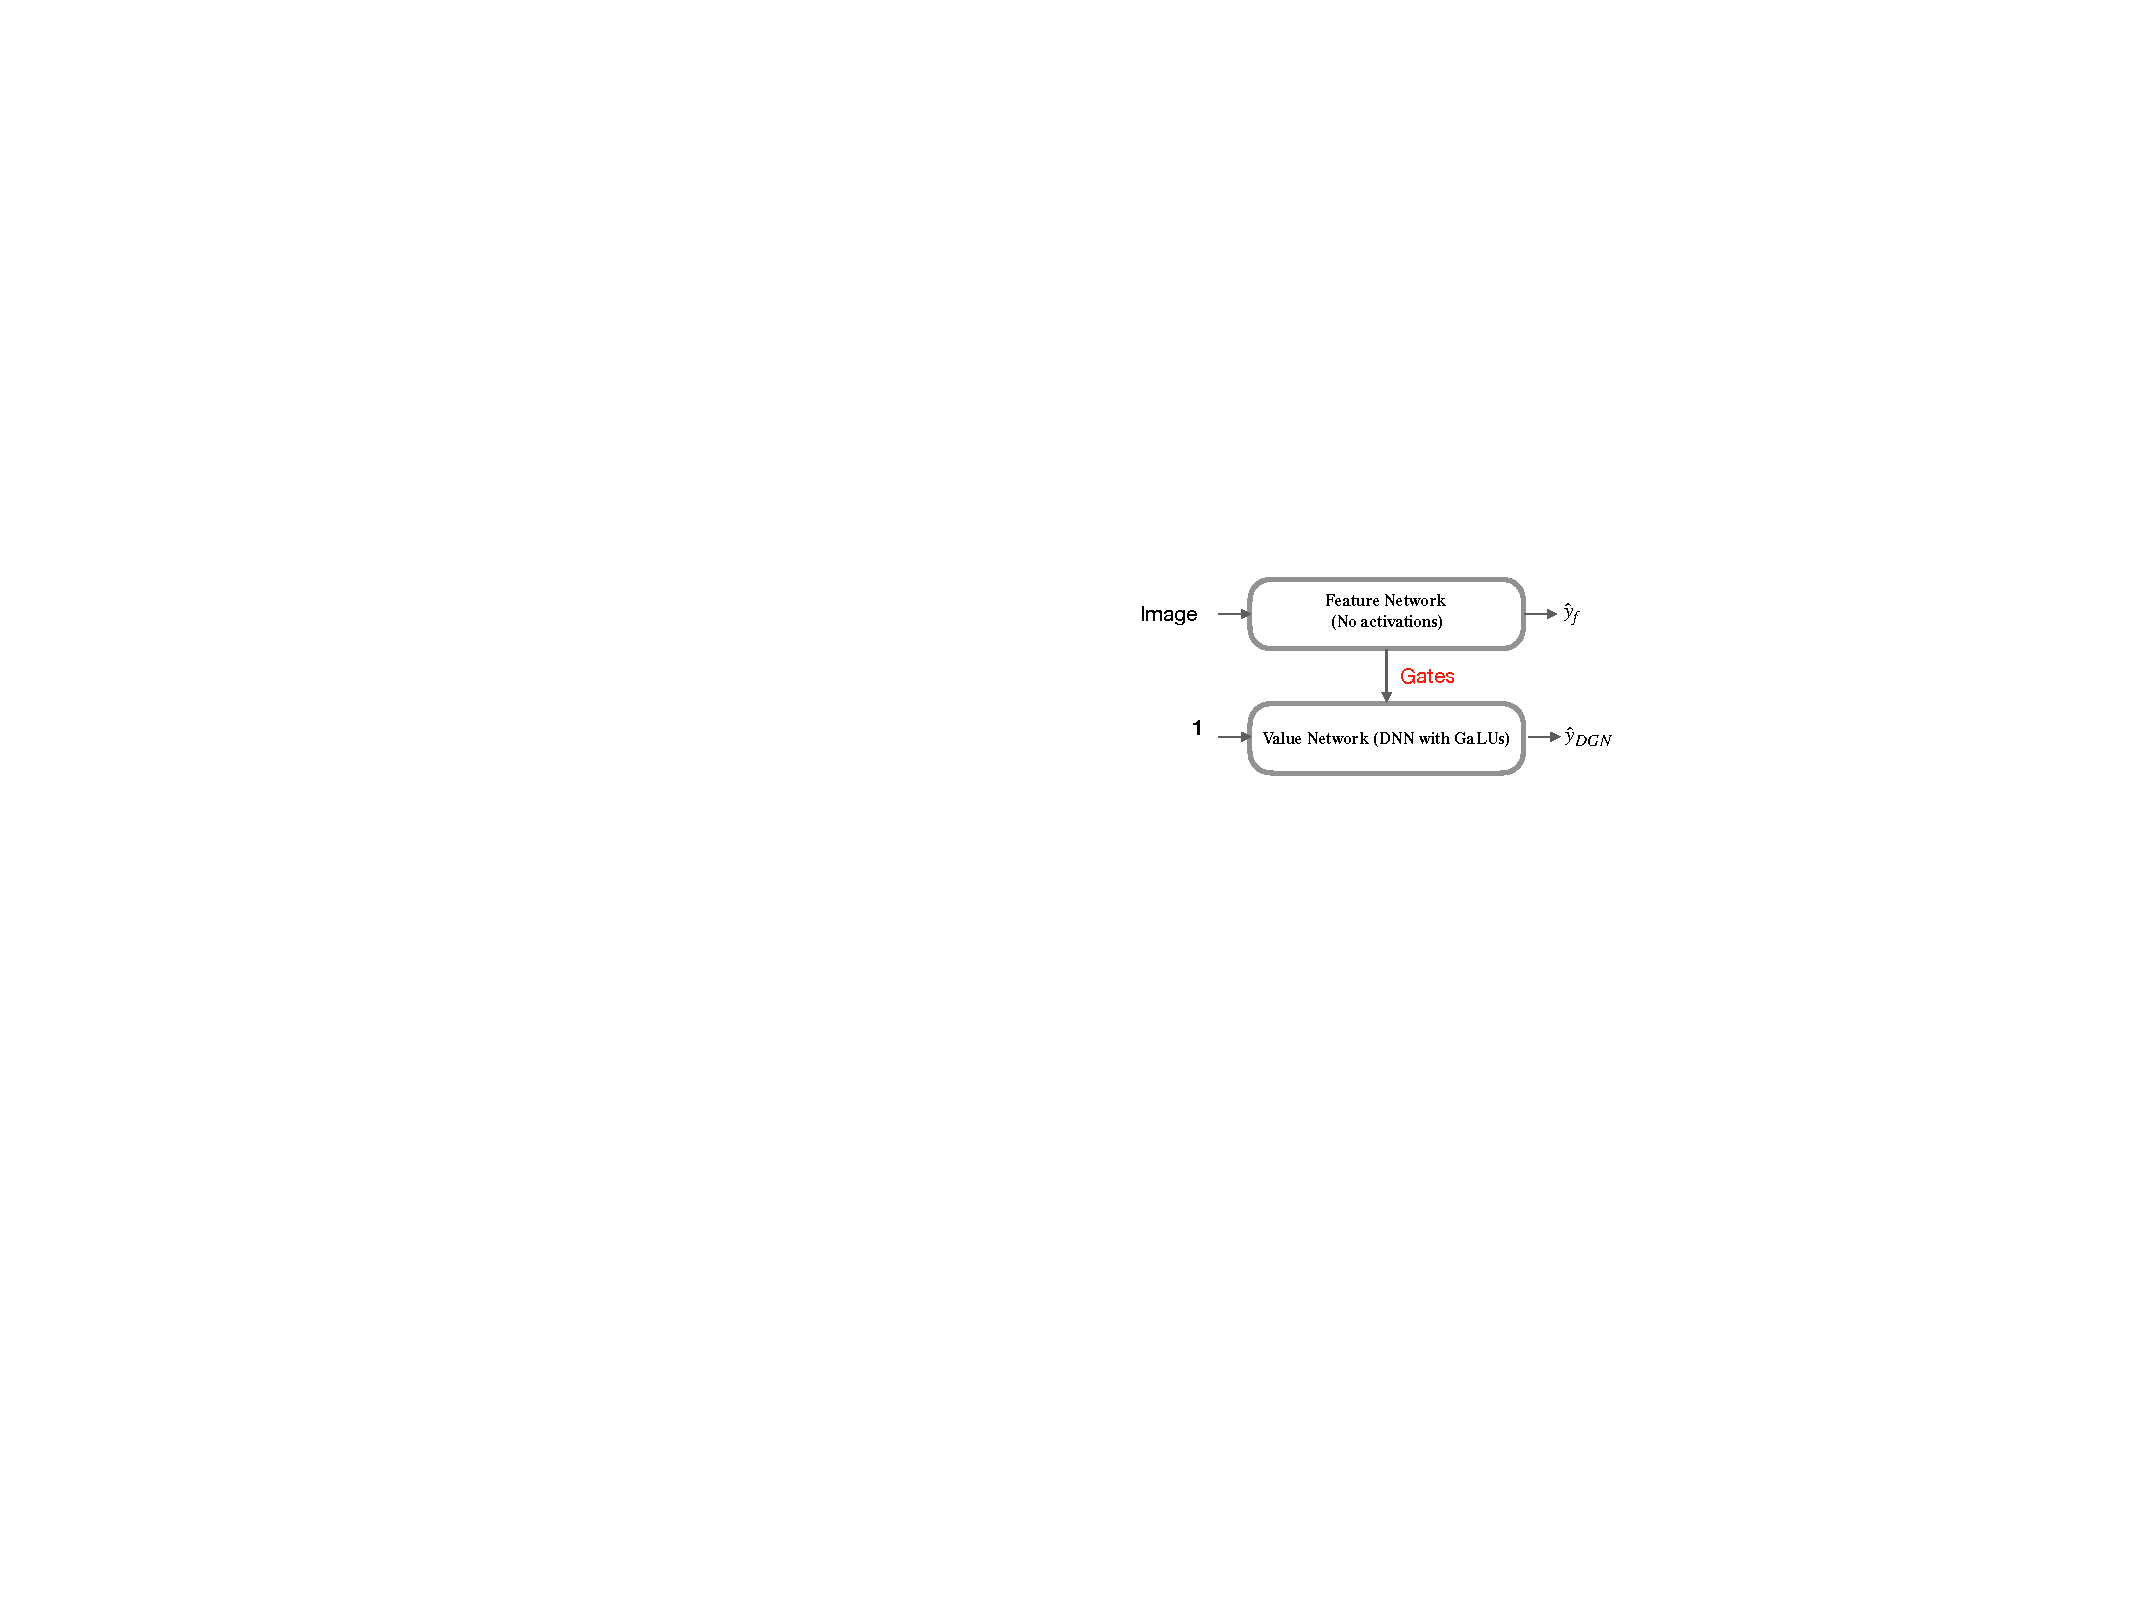
\includegraphics[scale=0.5]{figs/dgn-linear.pdf}
}
\end{minipage}
\begin{minipage}{0.4\columnwidth}
\begin{tabular}{rcc}
\toprule
&VGG19 & ResNet\\
Standard DNN&93.4\tiny{$\pm$0.1} &93.0\tiny{$\pm$0.1} \\
\texttt{DGN-No-Act}&91.7\tiny{$\pm$0.1}&90.9\tiny{$\pm$0.1} \\
\bottomrule
\end{tabular}
\end{minipage}
\caption{\small On the left is the \texttt{DGN-No-Act}. On right is $\%$ test accuracy on CIFAR-10, averaged over $5$ runs (best in each run). Optimiser: SGD with momentum of 0.9 (the learning rate and schedule are in the Appendix).}
\label{fig:dgn-no-act}
\end{figure}
\begin{comment}
\begin{wrapfigure}{r}{0.3\textwidth}
\resizebox{0.3\columnwidth}{!}{
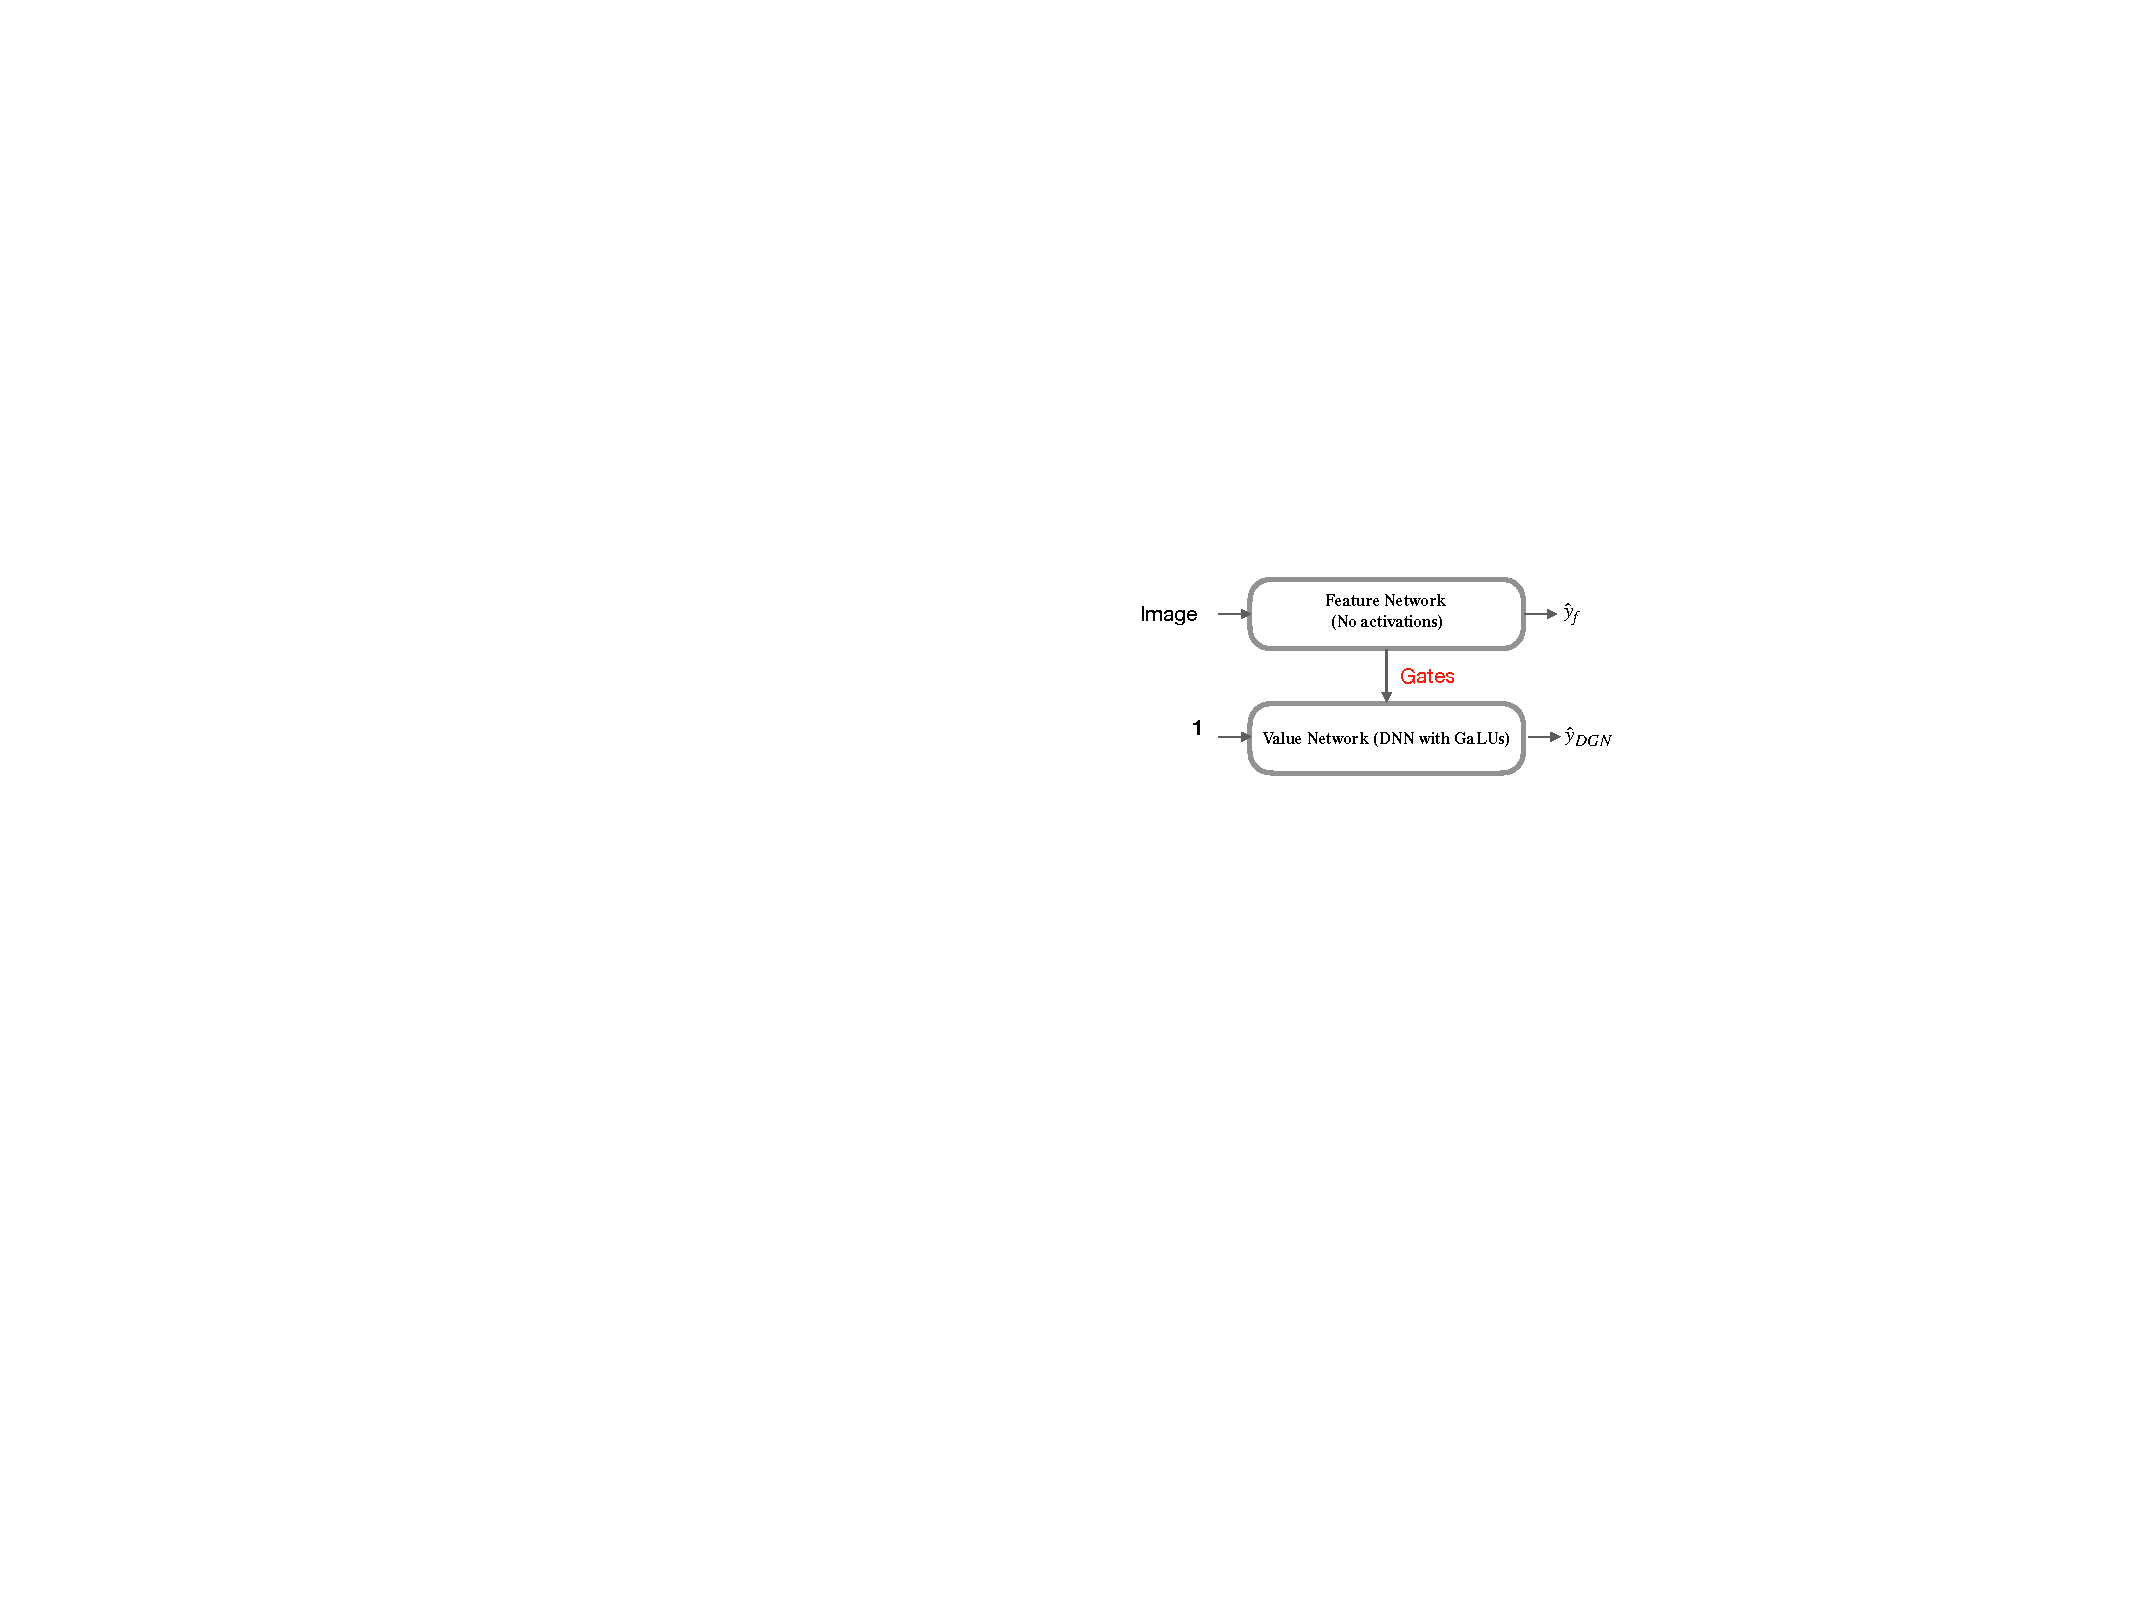
\includegraphics[scale=0.5]{figs/dgn-linear.pdf}
}
\end{wrapfigure}
\end{comment}
We used the DGN setup to answer the question `what is learnt in a DNN with ReLUs'. We now ask: `What happens if we remove activations (i.e., replace it with identity activations) from the feature network of a DGN?'-- let us call this the \texttt{DGN-No-Act}. If the activations are removed from the feature network, then feature generation will no longer be hidden, i.e., it will only be in terms of transformations such as matrix multiplication, pooling and scale/mean correction (in the case of batch norm), all of which have concrete `image processing'  interpretations. The gates in \texttt{DGN-No-Act} are derived (as usual) from the pre-activations of the identity activations in the feature network. We use soft-gating $G(q)=\frac{1}{1+\exp({-\beta\cdot q})}$, with $\beta=10$.  The value network in the \texttt{DGN-No-Act} has the same functionality, i.e., it learns the NPV. We constructed two such \texttt{DGN-No-Act}s based on standard architectures (VGG19 [\citenum{vgg}] and a ResNet[\citenum{davidnet}]), wherein, the standard architecture is used in feature network (without ReLU) and in the value network with ReLU replaced by GaLU. Both these \texttt{DGN-No-Act}s gave more than $90\%$ test accuracy on CIFAR-10 (see \Cref{fig:dgn-no-act}).

%We answered this question using the DGN setup, where the DNN with ReLU which we want to study is the feature network, and we measured the performance by training the value network. 
%Based on the insights obtained from \Cref{th:main}, especially those on the roles of feature and value networks, and further experiments on how gate learning happens,